% !TeX program = xelatex
% !TeX encoding = UTF-8
% !TeX TXS-program:compile = txs:///xelatex | txs:///xelatex
\documentclass[aspectratio=169, table, 12pt]{beamer}
% Preamble bersama seluruh slide mata kuliah ini.
% Dipanggil dari slides/sessionXX/sessionXX.tex tepat sesudah baris
% \documentclass[aspectratio=169, table, 12pt]{beamer}
% Paket tambahan yang hanya dibutuhkan satu sesi ditulis di berkas sesi itu.

\usepackage{colortbl}
\usepackage{xcolor}
\usepackage{listings}
\usepackage{tabularx}
\usepackage{booktabs}
\usepackage{tikz}
\usepackage{pgfplots}
\pgfplotsset{compat=1.18}
\usetikzlibrary{arrows.meta, positioning, calc, fit, shapes.geometric,
	shapes.multipart, backgrounds, matrix, chains, trees}

\makeatletter
\def\input@path{{../theme/}}
\makeatother
\graphicspath{{../theme/}{../../figures/}}
\usetheme{Pradita}

\definecolor{praditagreen}{RGB}{37, 113, 71}

% Tema membuat garis tabel berwarna putih. Dikembalikan agar tabel terbaca.
\arrayrulecolor{black}
\setlength{\arrayrulewidth}{0.5pt}

\lstdefinelanguage{yaml}{
	basicstyle=\ttfamily\scriptsize,
	keywordstyle=\color{blue}\bfseries,
	commentstyle=\color{gray}\itshape,
	stringstyle=\color{red},
	showstringspaces=false,
	breaklines=true,
	frame=lines,
	numbers=none,
	backgroundcolor=\color{lightgray!10},
	tabsize=2,
	morecomment=[l]{\#}
}

\lstdefinelanguage{json}{
	basicstyle=\ttfamily\scriptsize,
	stringstyle=\color{red},
	commentstyle=\color{gray},
	breaklines=true,
	showstringspaces=false,
	tabsize=2,
	numbers=none,
	frame=lines,
	backgroundcolor=\color{lightgray!10},
	string=[s]{"}{"}
}

\lstdefinelanguage{bash}{
	keywords={},
	basicstyle=\ttfamily\scriptsize,
	ndkeywords={docker, kubectl, helm, curl, git, terraform},
	ndkeywordstyle=\color{purple}\bfseries,
	sensitive=true,
	commentstyle=\color{gray},
	numbers=none,
	breaklines=true,
	frame=lines,
	backgroundcolor=\color{lightgray!10},
	tabsize=2,
	comment=[l]{\#},
	showstringspaces=false
}

\lstdefinelanguage{http}{
	keywords={GET, POST, PUT, PATCH, DELETE, HEAD, OPTIONS, HTTP},
	basicstyle=\ttfamily\scriptsize,
	keywordstyle=\color{blue}\bfseries,
	sensitive=true,
	numbers=none,
	breaklines=true,
	frame=lines,
	backgroundcolor=\color{lightgray!10},
	tabsize=2,
	showstringspaces=false
}

\subtitle{IT40613 · Digital Platform \& API Economy}
\author{\textbf{Alfa Yohannis}}


\title{\Huge Keamanan API:\\ \vspace{10pt} OAuth 2.0 dan OWASP}
\date{Pertemuan 06}

\begin{document}
\frame{\titlepage}

\begin{frame}
  \frametitle{Isi Pertemuan}
  \vspace{14pt}
  \begin{columns}[t]
    \column{0.5\textwidth}
    {\small\tableofcontents[sections={1-4}]}

    \column{0.5\textwidth}
    {\small\tableofcontents[sections={5-9}]}
  \end{columns}
\end{frame}

\begin{frame}{\hfill}
  \centering
  \Huge{\textbf{Kredensialnya sah.\\Vendornya resmi.\\Mengapa rekam medis\\tetap terbaca?}}
\end{frame}

\section{Tujuan dan Konteks}

\begin{frame}{{\Large Tujuan Pembelajaran}}
  \vspace{10pt}
  \begin{itemize}
    \item Membedakan autentikasi dan otorisasi pada API, serta peran \textit{API key}, token, dan \textit{scope}.
    \item Menjelaskan alur OAuth (\textit{Open Authorization}) 2.0 yang umum dipakai aplikasi dan mitra pada tingkat konsep.
    \item Menilai risiko keamanan integrasi yang berjalan dengan OWASP (\textit{Open Worldwide Application Security Project}) API Security Top 10 edisi 2023.
  \end{itemize}
\end{frame}

\begin{frame}{{\Large Diagram Konsep Bab 6}}
  \centering
  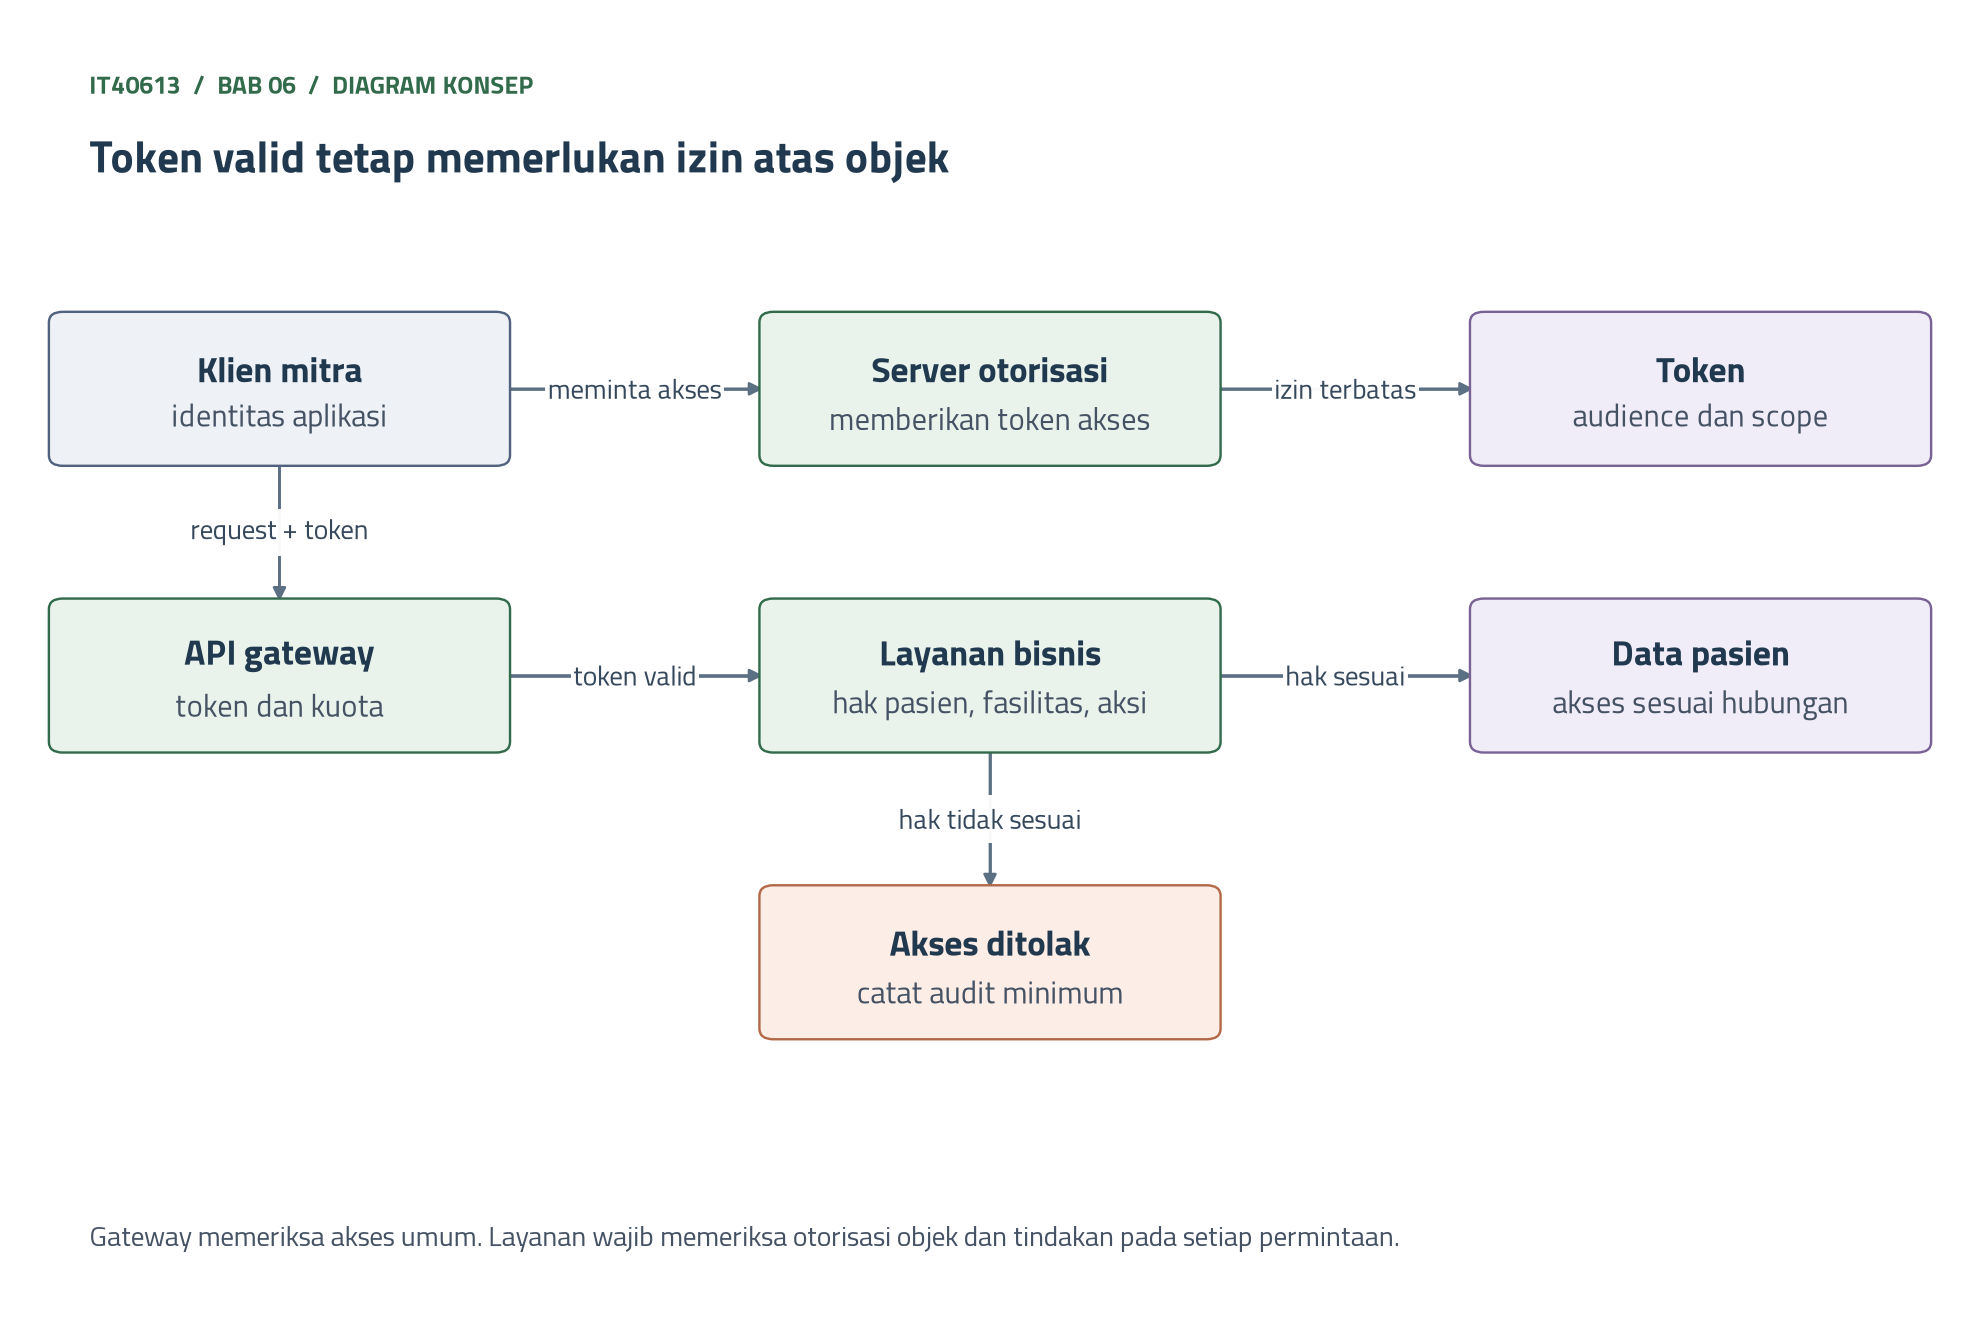
\includegraphics[width=0.96\textwidth,height=0.77\textheight,keepaspectratio]{../../figures/ch06-diagram-konsep.png}
\end{frame}

\section{Pola Insiden}

\begin{frame}{\hfill}
  \centering
  \Huge{\textbf{Pola Insiden Kebocoran\\Data Lewat API}}
\end{frame}

\begin{frame}{{\Large Risiko Muncul Saat Akses Melebihi Kewenangan}}
  \vspace{10pt}
  \begin{itemize}
    \item Kemampuan dan data diekspos melebihi kewenangan pemanggil.
    \item Asalnya: otorisasi objek lemah, autentikasi salah, konsumsi berlebihan, dan kepercayaan berlebih pada pihak ketiga.
    \item Jalur API dirancang untuk dipanggil mesin dalam jumlah besar.
    \item Daftar OWASP memberi pertanyaan, bukan bukti penyebab.
  \end{itemize}
  \vspace{6pt}
  {\small Analogi: kartu gedung menjawab siapa yang masuk, kunci lemari menjawab arsip mana yang boleh dibuka.}
\end{frame}

\begin{frame}{{\Large Dua Insiden dari Laporan Publik}}
  \small
  \begin{tabularx}{\textwidth}{>{\raggedright\arraybackslash}p{2.2cm}
      >{\raggedright\arraybackslash}X >{\raggedright\arraybackslash}p{3.1cm} >{\raggedright\arraybackslash}X}
    \hline
    \textbf{Insiden} & \textbf{Jalur} & \textbf{Waktu} & \textbf{Pelajaran} \\ \hline
    T-Mobile, 2022 sampai 2023 & Satu API, tanpa otorisasi, sekitar 37 juta akun & Sekitar 25 November sampai 5 Januari: 41 hari & Lama berjalan tanpa terlihat \\ \hline
    Salesloft Drift, 2025 & Token OAuth curian milik aplikasi pihak ketiga & Paling awal 8 Agustus, dicabut 20 Agustus: 12 hari & Platform kuat tetap kehilangan data lewat token mitra \\ \hline
  \end{tabularx}

  \vspace{8pt}
  Banyak akun T-Mobile tidak memuat seluruh bidang data. Laporan Drift menegaskan masalahnya bukan celah pada platform inti Salesforce.
\end{frame}

\begin{frame}{{\Large Lima Unsur yang Diperiksa}}
  \footnotesize
  \begin{tabularx}{\textwidth}{>{\raggedright\arraybackslash}p{2.1cm}
      >{\raggedright\arraybackslash}X >{\raggedright\arraybackslash}X >{\raggedright\arraybackslash}p{1.7cm}}
    \hline
    \textbf{Unsur} & \textbf{Pertanyaan} & \textbf{Kegagalan yang umum} & \textbf{Butir OWASP} \\ \hline
    Identitas & Siapa pemanggil, apakah buktinya masih sah? & Kredensial dipakai bersama, masa berlaku tidak diperiksa & API2 \\ \hline
    Kewenangan & Objek, bidang, dan aksi mana yang boleh? & Token sah membaca pasien lain & API1, API3, API5 \\ \hline
    Konsumsi & Berapa banyak yang boleh diambil? & Data ditarik terus tanpa batas & API4, API6 \\ \hline
    Inventaris & Jalur apa yang hidup, siapa pemiliknya? & Versi lama aktif, aliran data tidak tercatat & API9 \\ \hline
    Kepercayaan & Apakah masukan pihak ketiga diperiksa? & Respons vendor diterima tanpa validasi & API10 \\ \hline
  \end{tabularx}

  \vspace{6pt}
  \small Enkripsi tidak menjawab kelimanya. Misalkan 1 persen dari 1.100 hasil salah ID: 11 hasil per bulan tetap diteruskan.
\end{frame}

\begin{frame}{{\Large Kasus Medikara: Insiden Vendor 2025 (Data Latihan)}}
  \vspace{6pt}
  \begin{itemize}
    \item Misalkan akun dukungan vendor masih aktif setelah kontrak pekerjaan selesai.
    \item Akun itu memanggil API bawaan Sistem Informasi Manajemen Rumah Sakit (SIMRS) di 2 rumah sakit: 155 kali per malam, 8 malam, 1.240 rekam kunjungan.
    \item Semua panggilan membawa kredensial sah, sehingga autentikasi berhasil.
    \item Diketahui pada hari ke-11, lewat keluhan pasien.
    \item Catatan rinci disimpan 7 hari: 620 rekam dapat ditelusuri, 620 rekam tidak.
  \end{itemize}
\end{frame}

\section{Autentikasi dan Otorisasi}

\begin{frame}{{\Large Identitas dan Hak adalah Dua Pertanyaan}}
  \vspace{10pt}
  \begin{itemize}
    \item Autentikasi memeriksa identitas. Otorisasi memutuskan tindakan yang diizinkan.
    \item Kode 401: identitas belum terbukti, misalnya token kedaluwarsa. Kode 403: terbukti, tetapi tidak berhak.
    \item Token akses membawa hak berjangka. Token \textit{bearer} dipakai pihak yang memegangnya, sehingga dijaga seperti kunci.
    \item \textit{Audience} token adalah layanan tujuan, berbeda dari audiens API pada Bab 4.
  \end{itemize}
  \vspace{6pt}
  {\small Analogi: kartu anggota perpustakaan menunjukkan keanggotaan, izin petugas menentukan arsip yang boleh dipinjam.}
\end{frame}

\begin{frame}{{\Large Empat Pemeriksaan pada Satu Permintaan}}
  \centering
  \eadiagram{../../figures/ch06-lapis-pemeriksaan.tex}
\end{frame}

\begin{frame}{{\Large Tiap Bukti Menjawab Satu Pertanyaan}}
  \small
  \begin{tabularx}{\textwidth}{>{\raggedright\arraybackslash}p{1.9cm}
      >{\raggedright\arraybackslash}X >{\raggedright\arraybackslash}X >{\raggedright\arraybackslash}p{2.6cm}}
    \hline
    \textbf{Bukti} & \textbf{Yang dijawab} & \textbf{Yang tidak dijawab} & \textbf{Yang dilakukan} \\ \hline
    \textit{API key} & Aplikasi atau proyek mana & Pengguna mana, pasien mana & Lindungi dan rotasi \\ \hline
    Token akses & Hak apa, sampai kapan, untuk layanan mana & Apakah objek ini termasuk hubungan layanan & Periksa masa berlaku dan \textit{audience} \\ \hline
    \textit{Scope} & Jenis aksi & Pasien dan fasilitas mana & Beri sekecil mungkin \\ \hline
    Objek pasien & Hubungan layanan & Apakah tujuannya sah & Periksa pada server \\ \hline
  \end{tabularx}
\end{frame}

\begin{frame}{{\Large Contoh Berangka: Scope, Kredensial, Masa Berlaku}}
  \vspace{6pt}
  \begin{itemize}
    \item 240 hasil per hari untuk 40 klinik: 6 hasil per klinik. Hanya memeriksa \textit{scope} berarti 234 hasil lain terbuka.
    \item Misalkan kredensial dipakai bersama 40 klinik, 2 jam per klinik: Rp4,8 juta.
    \item Dengan identitas per mitra: satu klinik, Rp120.000, jejak jelas.
    \item Misalkan bocor 30 hari, kuota 300: 9.000 panggilan. Token 15 menit: paling banyak 300.
    \item Rahasia klien yang dicuri tetap menghasilkan token baru, sehingga tetap dirotasi.
  \end{itemize}
\end{frame}

\section{OAuth 2.0}

\begin{frame}{\hfill}
  \centering
  \Huge{\textbf{OAuth 2.0:\\Peran dan Dua Alur Utama}}
\end{frame}

\begin{frame}{{\Large Empat Peran OAuth 2.0}}
  \small
  \begin{tabularx}{\textwidth}{>{\raggedright\arraybackslash}p{4.2cm}
      >{\raggedright\arraybackslash}X >{\raggedright\arraybackslash}p{3.4cm}}
    \hline
    \textbf{Peran} & \textbf{Arti} & \textbf{Contoh Medikara} \\ \hline
    Pemilik sumber daya (\textit{resource owner}) & Pihak yang dapat memberi akses & Pasien atau organisasi \\ \hline
    Klien (\textit{client}) & Aplikasi yang meminta akses & Medikara+, sistem laboratorium \\ \hline
    Server otorisasi (\textit{authorization server}) & Menerbitkan token & Layanan identitas Medikara \\ \hline
    Server sumber daya (\textit{resource server}) & Melayani data bila sah & API hasil laboratorium \\ \hline
  \end{tabularx}

  \vspace{8pt}
  Analogi: surat kuasa membatasi tindakan penerima kuasa, dan loket tetap memeriksa isi surat.
\end{frame}

\begin{frame}{{\Large Alur Client Credentials}}
  \centering
  \eadiagram{../../figures/ch06-alur-client-credentials.tex}
\end{frame}

\begin{frame}{{\Large Alur Authorization Code dengan PKCE}}
  \centering
  \eadiagram{../../figures/ch06-alur-pkce.tex}
\end{frame}

\begin{frame}{{\Large Contoh Berangka Dua Alur}}
  \vspace{6pt}
  \begin{itemize}
    \item INT-06, 3 laboratorium, misalkan token 15 menit: paling banyak 48 token per laboratorium, 144 token per hari.
    \item Satu laboratorium dicabut: token terakhir mati paling lama 15 menit, dua lainnya tidak terganggu.
    \item Ponsel adalah klien publik, sehingga rahasia yang ditanam dapat dibongkar.
    \item Misalkan 0,1 persen dari 28.000 sesi kodenya tertangkap: 28 sesi. PKCE membuat kode itu tidak dapat ditebus.
    \item RFC 9700 mewajibkan \textit{Proof Key for Code Exchange} (PKCE) untuk klien publik.
  \end{itemize}
\end{frame}

\begin{frame}{{\Large Memilih Alur Menurut Pihak yang Diwakili}}
  \footnotesize
  \begin{tabularx}{\textwidth}{>{\raggedright\arraybackslash}X
      >{\raggedright\arraybackslash}p{3.0cm} >{\raggedright\arraybackslash}X >{\raggedright\arraybackslash}p{2.5cm}}
    \hline
    \textbf{Keadaan} & \textbf{Alur} & \textbf{Alasan} & \textbf{Contoh Medikara} \\ \hline
    Aplikasi server, tanpa pengguna & \textit{Client credentials} & Tidak ada pasien yang masuk, klien menjaga rahasia & INT-06, INT-07 \\ \hline
    Aplikasi mewakili pasien atau dokter & \textit{Authorization code} dengan PKCE & Sandi hanya masuk ke server otorisasi & Medikara+, INT-03 \\ \hline
    Aplikasi meminta sandi pasien & Tidak dipakai & RFC 9700 melarang alur sandi pemilik & Pola lama \\ \hline
    Token langsung lewat pengalihan & Dihindari & RFC 9700 menyarankan tidak memakai \textit{implicit} & Pola lama \\ \hline
  \end{tabularx}

  \vspace{6pt}
  \small INT-03: API privat menggantikan akun basis data yang membaca 140 tabel, kebutuhannya 2 tabel.
\end{frame}

\section{Identitas dan Persetujuan}

\begin{frame}{{\Large OpenID Connect Menambah Lapisan Identitas}}
  \small
  \begin{tabularx}{\textwidth}{>{\raggedright\arraybackslash}p{3.4cm}
      >{\raggedright\arraybackslash}X >{\raggedright\arraybackslash}X}
    \hline
    \textbf{Unsur} & \textbf{Token akses (OAuth 2.0)} & \textbf{\textit{ID Token} (OpenID Connect)} \\ \hline
    Yang dijawab & Apa yang boleh dilakukan klien & Siapa pengguna yang baru masuk \\ \hline
    Ditujukan kepada & Server sumber daya & Klien \\ \hline
    Dipakai untuk & Memanggil API & Memulai sesi masuk di aplikasi \\ \hline
    Salah pakai yang umum & Dijadikan bukti masuk & Dikirim ke API sebagai izin \\ \hline
  \end{tabularx}

  \vspace{8pt}
  Misalkan 12 dokter pindah per tahun, 3 aplikasi: tanpa identitas bersama ada 36 akun yang harus ditutup. Dengan satu server otorisasi cukup 12.
\end{frame}

\begin{frame}{{\Large Persetujuan Pemilik Data Punya Dua Lapis}}
  \vspace{6pt}
  \begin{itemize}
    \item UU 27/2022: data kesehatan adalah data pribadi spesifik (Pasal 4).
    \item Persetujuan eksplisit hanya satu dari enam dasar pemrosesan (Pasal 20).
    \item Permenkes 24/2022: isi rekam medis wajib dijaga kerahasiaannya (Pasal 32), dan pembukaannya terbatas sesuai kebutuhan (Pasal 33).
    \item Layar persetujuan mencatat izin pasien kepada satu klien.
    \item Layar belum tentu memadai sebagai dasar hukum.
  \end{itemize}
  \vspace{4pt}
  {\small Analogi: formulir izin tindakan berlaku untuk satu tindakan tertentu.}
\end{frame}

\begin{frame}{{\Large Layar Persetujuan dan Dasar Pemrosesan}}
  \footnotesize
  \begin{tabularx}{\textwidth}{>{\raggedright\arraybackslash}X
      >{\raggedright\arraybackslash}p{2.9cm} >{\raggedright\arraybackslash}p{2.0cm} >{\raggedright\arraybackslash}X}
    \hline
    \textbf{Situasi} & \textbf{Alur} & \textbf{Layar} & \textbf{Dasar yang diuji fungsi hukum} \\ \hline
    Pasien mengizinkan aplikasi pihak ketiga & \textit{Authorization code} dengan PKCE & Ada, per klien dan \textit{scope} & Persetujuan eksplisit \\ \hline
    Pasien memakai Medikara+ & \textit{Authorization code} dengan PKCE & Dicatat saat mendaftar & Perjanjian atau persetujuan \\ \hline
    Laboratorium mengirim hasil rujukan & \textit{Client credentials} & Tidak ada & Perjanjian dan persetujuan pasien untuk pengobatan \\ \hline
    INT-01, INT-02 ke pihak wajib & Spesifikasi pihak wajib & Tidak ada & Kewajiban hukum \\ \hline
  \end{tabularx}

  \vspace{6pt}
  \small INT-01: pemeriksaan kepesertaan tidak membuka isi rekam medis, sehingga 55.000 layar per bulan tidak menyelesaikan apa pun. Klaim memakai persetujuan saat registrasi (Permenkes 24/2022 Pasal 34 ayat (7)). Kolom terakhir adalah hipotesis, bukan pendapat hukum.
\end{frame}

\section{Profil Keamanan}

\begin{frame}{{\Large Praktik Utama RFC 9700}}
  \footnotesize
  \begin{tabularx}{\textwidth}{>{\raggedright\arraybackslash}p{2.4cm}
      >{\raggedright\arraybackslash}X >{\raggedright\arraybackslash}X}
    \hline
    \textbf{Praktik} & \textbf{Isi RFC 9700} & \textbf{Arti bagi Medikara} \\ \hline
    Alur aman & Klien publik wajib PKCE, klien rahasia dianjurkan & Medikara+ dan portal mitra memakai PKCE \\ \hline
    Pengalihan & Wajib dicocokkan secara persis & Alamat terdaftar per klien \\ \hline
    Alur lama & Alur sandi dilarang, \textit{implicit} sebaiknya tidak & Vendor peminta sandi masuk daftar kesenjangan \\ \hline
    Token curian & Sebaiknya terikat pengirim: mTLS atau DPoP & Token API mitra diikat ke kunci klien \\ \hline
    Hak minimum & Sekecil kebutuhan, dibatasi \textit{audience} & Token API hasil tidak berlaku di API tagihan \\ \hline
    \textit{Refresh token} & Klien publik: terikat pengirim atau dirotasi & Medikara+ merotasi \textit{refresh token} \\ \hline
  \end{tabularx}

  \vspace{4pt}
  mTLS: \textit{mutual Transport Layer Security}. DPoP: \textit{Demonstrating Proof of Possession}.
\end{frame}

\begin{frame}{{\Large OAuth 2.1 dan FAPI 2.0}}
  \vspace{10pt}
  \begin{itemize}
    \item OAuth 2.1 masih \textit{Internet-Draft}: draf ke-16, diperbarui 2 September 2026.
    \item \textit{Financial-grade API} (FAPI) 2.0 dirancang untuk data bernilai tinggi dan sensitif, termasuk kesehatan elektronik.
    \item FAPI 2.0 hanya mendukung klien rahasia dan token terikat pengirim, serta mewajibkan PKCE S256.
    \item Medikara+ di ponsel adalah klien publik, sehingga perlu perubahan arsitektur.
    \item Spesifikasi BPJS Kesehatan dan SATUSEHAT ditentukan pihak wajib (Bab 7).
  \end{itemize}
\end{frame}

\begin{frame}{{\Large Peta Keputusan Alur dan Profil}}
  \centering
  \eadiagram{../../figures/ch06-peta-keputusan.tex}
\end{frame}

\begin{frame}{{\Large Contoh Berangka: Biaya dan Kesiapan Mitra}}
  \vspace{10pt}
  \begin{itemize}
    \item Misalkan profil ketat menambah 20 persen: Rp9 juta dari Rp45 juta per antarmuka.
    \item Pada 20 sambungan aktif: tambah Rp180 juta per tahun.
    \item Misalkan hanya 5 sambungan data klinis: tambah Rp45 juta per tahun, seperempatnya.
    \item Misalkan 12 dari 40 klinik mampu DPoP: 28 klinik tertahan, 168 dari 240 hasil tetap lewat telepon.
    \item Kesenjangan dicatat dengan pemilik dan tenggat, bukan dilabeli patuh.
  \end{itemize}
\end{frame}

\section{OWASP API Security}

\begin{frame}{\hfill}
  \centering
  \Huge{\textbf{OWASP API Security\\Top 10 Edisi 2023}}
\end{frame}

\begin{frame}{{\Large Sepuluh Butir: API1 sampai API5}}
  \footnotesize
  \begin{tabularx}{\textwidth}{>{\raggedright\arraybackslash}p{4.3cm}
      >{\raggedright\arraybackslash}X >{\raggedright\arraybackslash}X}
    \hline
    \textbf{Butir} & \textbf{Arti sederhana} & \textbf{Contoh Medikara} \\ \hline
    API1 \textit{Broken Object Level Authorization} (BOLA) & Mengganti ID, memperoleh objek pihak lain & Token klinik A membaca pasien klinik B \\ \hline
    API2 \textit{Broken Authentication} & Bukti identitas lemah & Kredensial dipakai bersama \\ \hline
    API3 \textit{Broken Object Property Level Authorization} & Melihat bidang yang bukan haknya & Rekap perusahaan memuat diagnosis \\ \hline
    API4 \textit{Unrestricted Resource Consumption} & Tanpa batas laju, ukuran, biaya & Klinik menarik ribuan hasil per jam \\ \hline
    API5 \textit{Broken Function Level Authorization} & Akun biasa memakai fungsi peran lain & Akun klinik memakai fungsi hapus hasil \\ \hline
  \end{tabularx}
\end{frame}

\begin{frame}{{\Large Sepuluh Butir: API6 sampai API10}}
  \footnotesize
  \begin{tabularx}{\textwidth}{>{\raggedright\arraybackslash}p{4.3cm}
      >{\raggedright\arraybackslash}X >{\raggedright\arraybackslash}X}
    \hline
    \textbf{Butir} & \textbf{Arti sederhana} & \textbf{Contoh Medikara} \\ \hline
    API6 \textit{Unrestricted Access to Sensitive Business Flows} & Alur sah dipakai berlebihan secara otomatis & Program otomatis memborong slot dokter \\ \hline
    API7 \textit{Server Side Request Forgery} & Server dipaksa memanggil alamat dari pemanggil & Fitur ambil rujukan memanggil server internal \\ \hline
    API8 \textit{Security Misconfiguration} & Konfigurasi longgar & Pesan \textit{error} membuka rincian SIMRS \\ \hline
    API9 \textit{Improper Inventory Management} & API atau aliran data tanpa catatan & INT-10: 12 sambungan tanpa pemilik \\ \hline
    API10 \textit{Unsafe Consumption of APIs} & Data pihak ketiga dipercaya tanpa periksa & Hasil laboratorium langsung masuk SIMRS \\ \hline
  \end{tabularx}
\end{frame}

\begin{frame}{{\Large Membaca Daftar OWASP dengan Kritis}}
  \vspace{10pt}
  \begin{itemize}
    \item API1 (BOLA): mudah dieksploitasi, tersebar luas, mudah dideteksi, karena server mengandalkan ID dari klien.
    \item Edisi 2023 tidak berbasis data: prevalensi berasal dari konsensus tim.
    \item Penilaian OWASP tidak memperhitungkan dampak nyata pada bisnis, sehingga organisasi tetap menilainya.
    \item API1 bertanya pasien mana, API3 bidang mana, API5 fungsi mana.
    \item API10 tentang data yang masuk dari pihak ketiga, bukan semua masalah vendor.
  \end{itemize}
\end{frame}

\begin{frame}{{\Large Matriks Dampak dan Kemungkinan}}
  \centering
  \eadiagram{../../figures/ch06-matriks-risiko.tex}
\end{frame}

\begin{frame}{{\Large Contoh Register Risiko (Data Latihan)}}
  \scriptsize
  \begin{tabularx}{\textwidth}{>{\raggedright\arraybackslash}p{1.0cm}
      >{\raggedright\arraybackslash}p{1.5cm} >{\raggedright\arraybackslash}p{0.9cm} >{\raggedright\arraybackslash}X
      >{\raggedright\arraybackslash}p{0.7cm} >{\raggedright\arraybackslash}p{2.1cm}}
    \hline
    \textbf{ID} & \textbf{Integrasi} & \textbf{Butir} & \textbf{Temuan} & \textbf{Skor} & \textbf{Status bukti} \\ \hline
    RA-01 & INT-03 & API3 & Akun vendor membaca 140 tabel, kebutuhan 2 tabel & 9 & Terverifikasi \\ \hline
    RA-02 & INT-03 & API1 & API bawaan di 2 rumah sakit diduga tidak memeriksa hubungan layanan & 9 & Hipotesis \\ \hline
    RA-03 & INT-10 & API9 & 12 sambungan resep tanpa pemilik dan catatan aliran data & 6 & Belum terverifikasi \\ \hline
    RA-04 & INT-07 & API3 & Rekap 36 perusahaan memuat data karyawan lebih dari kebutuhan & 6 & Terverifikasi \\ \hline
    RA-05 & INT-06 & API2 & Hasil 3 laboratorium lewat surel, pengirim tidak diuji & 4 & Wawancara \\ \hline
    RA-06 & INT-02 & API10 & Jawaban SATUSEHAT tidak diperiksa, 4 persen belum terkirim & 4 & Terverifikasi \\ \hline
    RA-07 & Usulan API hasil & API4 & Kuota 300 per hari per klinik belum diterapkan & 2 & Rancangan \\ \hline
  \end{tabularx}

  \vspace{6pt}
  \footnotesize Skor tinggi dengan status hipotesis berarti uji berizin, bukan temuan terbukti. Uji hanya pada sistem sendiri atau berizin tertulis.
\end{frame}

\section{Pembatasan dan Pencatatan}

\begin{frame}{{\Large Laju, Kuota, dan Akibatnya}}
  \vspace{10pt}
  \begin{itemize}
    \item \textit{Rate limiting} membatasi laju, kuota membatasi jumlah dalam periode.
    \item Misalkan penyalahgunaan 5 permintaan per detik: 216.000 dalam 12 jam tanpa batas.
    \item Batas 1 permintaan per detik: 43.200. Kuota 300: berhenti setelah 60 detik, lalu 429.
    \item Kapasitas 40 klinik tetap 12.000 panggilan per hari.
    \item Pola 155 panggilan per malam lolos dari kuota: yang menghentikan adalah hak atas objek.
  \end{itemize}
\end{frame}

\begin{frame}{{\Large Isi Catatan Akses}}
  \small
  \begin{tabularx}{\textwidth}{>{\raggedright\arraybackslash}X >{\raggedright\arraybackslash}X}
    \hline
    \textbf{Dicatat} & \textbf{Tidak dicatat} \\ \hline
    ID permintaan dan waktu & Token akses dan rahasia klien \\ \hline
    Identitas klien dan akun & Sandi pengguna \\ \hline
    Operasi dan ID objek & Isi rekam medis dan hasil pemeriksaan \\ \hline
    Keputusan akses dan alasannya & Kunci enkripsi \\ \hline
  \end{tabularx}

  \vspace{8pt}
  Misalkan 444.000 catatan per bulan: 2,7 GB per tahun. Bila isi ikut dicatat: 266,4 GB, dan \textit{log} menjadi salinan kedua rekam medis.

  \vspace{4pt}
  UU 27/2022 Pasal 46: pemberitahuan paling lambat 3 $\times$ 24 jam, memuat data yang terungkap, kapan, dan bagaimana.
\end{frame}

\section{Aktivitas, Ringkasan, dan Latihan}

\begin{frame}{{\Large Aktivitas: Penilaian Risiko Keamanan API}}
  \vspace{6pt}
  \begin{itemize}
    \item Pilih tiga integrasi dari peta Bab 5 dengan akibat terbesar bila disalahgunakan.
    \item Isi daftar periksa OWASP per integrasi, tanpa menguji sistem luar.
    \item Kumpulkan bukti dari sumber berizin, tandai yang masih hipotesis.
    \item Beri nilai dampak dan kemungkinan, lalu jalankan \texttt{hitung-risiko-api.py}.
    \item Tetapkan pemilik, kontrol sementara, dan tanggal tinjau untuk temuan tinggi.
  \end{itemize}
\end{frame}

\begin{frame}{{\Large Aktivitas: Peran, Luaran, dan Kriteria}}
  \vspace{4pt}
  \begin{itemize}
    \item Hukum, kesehatan, bisnis: dampak pada pasien, kepatuhan, reputasi.
    \item Teknis: bukti autentikasi, akses per objek, dan pencatatan.
    \item Luaran untuk tonggak C2: lembar periksa, register risiko, catatan keputusan.
    \item Kriteria: konsep 25\%, keterlacakan bukti 30\%, alasan keputusan 30\%, keterbacaan 15\%.
    \item Berkas: \berkas{sources/chapter06/README.md}.
  \end{itemize}
  \vspace{4pt}
  {\small Pemindaian, uji beban, dan uji hak akses hanya untuk sistem sendiri atau yang sudah berizin tertulis.}
\end{frame}

\begin{frame}{{\Large Ringkasan}}
  \vspace{10pt}
  \begin{itemize}
    \item Risiko API muncul ketika akses melebihi kewenangan pemanggil.
    \item \textit{API key}, token, dan \textit{scope} tidak menjawab pasien yang mana.
    \item \textit{Client credentials} untuk aplikasi server, PKCE untuk aplikasi yang mewakili pasien.
    \item OWASP memberi pertanyaan, bukan vonis dan bukan prioritas.
    \item Pesan utama: token yang sah bukan izin atas semua data.
  \end{itemize}
\end{frame}

\begin{frame}{{\Large Latihan}}
  \vspace{10pt}
  \begin{enumerate}
    \item Jelaskan dengan contoh rekam medis mengapa \textit{Broken Object Level Authorization} menempati urutan pertama.
    \item Bandingkan pemakaian \textit{API key} dan OAuth 2.0 \textit{client credentials} untuk integrasi dengan laboratorium mitra.
    \item Kebocoran data Medikara pada 2025 terjadi lewat vendor. Tentukan dua butir OWASP API Security Top 10 yang paling relevan, lalu jelaskan alasannya.
  \end{enumerate}
\end{frame}

\end{document}
